\clubpenalty100000000
\widowpenalty100000000
\documentclass[svgnames,12pt]{scrartcl}

\usepackage{xltxtra,polyglossia}
\usepackage{graphicx}
\usepackage[round]{natbib}
\usepackage[table]{xcolor}
\usepackage{booktabs}
\usepackage{color, colortbl, multirow}
\usepackage{hyperref} 
\hypersetup{bookmarks=false,bookmarksnumbered,bookmarksopenlevel=5,bookmarksdepth=5,xetex,colorlinks=true,linkcolor=blue,citecolor=blue}

\setmainfont{Times New Roman}
\usepackage[all]{hypcap}
\usepackage{memhfixc}
\usepackage{tikz}
\usetikzlibrary{trees}
\usepackage{gb4e}  
\setmainlanguage{english}
\fontfamily{ptm}\selectfont

\setcitestyle{aysep={},citesep={,},notesep={:}}
%\newfontfamily\hana{HAN NOM A}
%\newcommand\Chinese[1]{{\hana #1}}
\newcommand\Comment[1]{\textcolor{red}{#1}}
\newfontfamily\phon[Mapping=tex-text,Ligatures=Common,Scale=MatchLowercase]{Charis SIL} 
\newcommand{\ipa}[1]{\textbf{{\phon\mbox{#1}}}} 
\newcommand{\grise}[1]{\cellcolor{lightgray}\textbf{#1}}
\newfontfamily\cn{HAN NOM A}%pour le chinois
\newcommand{\zh}[1]{{\cn#1}}

\title{Save the Trees: Why we need tree models in linguistic reconstruction (and when we should
apply them)}
%\author{Guillaume Jacques and Johann-Mattis List}  
%acknowledgements: Juho Pystynen, Mikhail Zhivlov, Nathan Hill, Mathieu Ségui, John Cowan, Simon Greenhill, Dmitry Nikolaev, Yoram Meroz, Tiago Tresoldi, Rémy Viredaz, Martin Kümmel
\begin{document}
\maketitle
\begin{abstract}
  \small
Scepticism against the tree model has a long tradition in historical linguistics.  Although scholars
have emphasized that the tree model and its longstanding counterpart, the wave theory, are not
necessarily incompatible, the opinion that family trees are unrealistic and should be completely abandoned from
historical linguistics has always enjoyed a certain popularity. This scepticism has further
increased with recently proposed techniques for data visualization which seem to confirm that we can 
study language history without trees.  In this paper, we show that family trees are not only a
logical but also a practical necessity in linguistic reconstruction. While the logical necessity of
the tree model follows directly from the basic assumptions underlying linguistic reconstruction, the
practical necessity of the tree-model follows from its implications for a realistic modeling of
language history, which always needs to involve a before and after of events.  In order to save the
trees from the critics, we show that the concrete arguments brought up in favor of
anachronistic wave models do not hold. In comparing the phenomenon of \emph{incomplete lineage
sorting} in biology with processes in linguistics, we show that data which does not seem to be
resolvable in trees may well be explained without turning to diffusion as an explanation. At the
same time, methodological limits in historical reconstruction may easily lead to an overestimation
of regularity, which may in turn surface as conflicting patterns when trying to reconstruct a
coherent phylogeny. 
  While acknowledging that not all
aspects of language history are tree-like, and that integrated models which capture both vertical
and lateral language relations may depict language history more realistically, we claim that all
models which claim that vertical language relations can be completely ignored are essentially wrong:
Either they silently still use family trees, or they only provide a static display of data and thus
fail to model temporal aspects of language history.
\end{abstract}
\section{Introduction}
All languages develop by descent with modification: linguistic material is transferred from
generation to generation of speakers, and slight modifications in pronunciation, denotation, and
grammar may sum up to changes which are so large that when two or more linguistic varieties have
been separated in some way, be it by geographical or political separation of their speakers, they
may become mutually incomprehensible. Not all linguistic material is necessarily inherited from the
parent generation. Linguistic material may easily be transferred across linguistic boundaries or
diffuse across similar speech varieties. This does, however, not change the fact that the primary
process by which languages are transmitted is the acquisition of a first language by children
(\citealt[61]{Ringe2002}, \citealt[27-48]{Hale2007}). That largely incomprehensible and different languages may share a common
genetic origin was one of the great insights of 19th century linguistics, and even if lateral forces
of diffusion may drastically change the shape of languages, this does not invalidate the crucial
role that vertical transmission plays in language history, and we follow \citet[347]{Labov2007} in
strictly distinguishing transmission of language via first-language-acquisition from diffusion via
contact as two distinct processes. 
 
In the following, we want to substantiate
this viewpoint. Starting from a brief overview on the historical debate between trees and waves in
the history of linguistics, we will introduce the core arguments of the new debate about trees and
waves, and then defend tree thinking in historical linguistics by showing that patterns which do not
look tree-like from a first sight may still be explained by a branching tree model, while on the
other hand patterns that look like common inheritance may go back to processes of
language contact, which are acknowledged by all proponents of the family tree model, and can thus not be used as arguments against the tree model. We
conclude that both tree- and non-tree-like processes need to be taken into account when trying to
draw a realistic scenario of language history. The logical and practical necessity of using both
models for tree-like and non-tree-like evolution shows that we cannot simply abandon the tree model
in historical linguistics, but should rather work on integrating vertical transmission and
horizontal diffusion in a common framework.
\section{Dendrophobia and Dendrophilia in Linguistics}
In order to get a clearer picture of the major arguments brought up to support or to dismiss the
family tree model it is useful to have a closer look at the origins of the tree model and the
discussions that it instigated. In the following, we will give a brief overview on the development
of tree thinking (``dendrophilia") and tree scepticism (``dendrophobia") in linguistics from its
beginnings up to today.
 
\subsection{Tree Thinking in Schleicher's Work}
Although not the first to draw language trees,\footnote{The first trees and networks depicting
language development date at least back to the 17th century (for details, see \citealt{List2016h},
\citealt{Morrison2016}, and \citealt{Sutrop2012}).} it was August Schleicher (1821-1866) who
popularized tree-thinking in linguistics. In two early papers from 1853
\citep{Schleicher1853,Schleicher1853a}, and numerous studies published thereafter (see, for example,
\citealt{Schleicher1861,Schleicher1863}), he propagated that the assumptions about language history
could be best `{illustrated by the image of a branching tree'
\citep[787]{Schleicher1853}.\footnote{Our translation, original text: `[Diese Annahmen, logisch
folgend aus den Ergebnissen der bisherigen Forschung,] lassen sich am besten unter dem Bilde eines
sich verästelnden Baumes anschaulich machen'.} Note that there was no notable influence by Darwin
here. It is more likely that Schleicher was influenced by \emph{stemmatics} (manuscript comparison,
see \citealt[8]{Hoenigswald1963}). Even today, historical linguistics has certain features that
resemble manuscript comparison much more closely than evolutionary biology. It seems that
Schleicher's enthusiasm for the drawing of language trees had quite an impact on Ernst Haeckel
(1834-1919, see \citealt{Sutrop2012}), since – as Schleicher pointed out himself
\citep[14]{Schleicher1863} – linguistic trees by then were explicit, pointing to concrete
languages, and not abstract, pointing to hypothetical taxa, like the one Darwin showed in his
Origins \citep{Darwin1859}.
 
Despite the seemingly radical idea to model language history as process of diversification
exclusively via branching and splitting, it is important to note that Schleicher was not a careless
proponent of tree thinking. Judging from his work we find many examples showing that he was aware of
potential problems resulting from the tree model. Thus, in his open letter to Haeckel, Schleicher,
taking Latin and its descendants as an example, explicitly pointed to problems of language mixing
which he compared to plant hybrids in biology, identifying it as a second factor leading to
differentiation \citep[18]{Schleicher1863}. 
In his earlier work, he mentioned language contact and
borrowing of linguistic features explicitly as a process characteristic for language history \citep[6]{Schleicher1861}, emphasizing the importance of
distinguishing borrowed from inherited traits in language classification \citep[30]{Schleicher1848}.
Following up the analogy with species evolution, Schleicher also pointed to the problem of finding
sharp borders between languages, dialects, and speech varieties (`Sprache, Dialekt, Mundarten und
Untermundarten'), which finds a counter-part in the distinction between species and
individuals \citep[21]{Schleicher1863}. Especially this last point clearly reflects
that Schleicher did not exclusively think that
language splits were a product of abrupt separation of speakers, and that he was aware of the
idealizing aspect of the \emph{Stammbaum}.

\subsection{Tree Scepticism in the Work of Schmidt and Schuchardt}
Schleicher's tree-thinking, however, did not last long in the world of historical linguistics.
By the beginning of the 1870s, Hugo Schuchardt (1842-1927) and Johannes Schmidt (1843-1901) published
critical views, claiming that vertical descent is not all what language evolution is about
\citep{Schmidt1872,Schuchardt1870}. While Schmidt remained very vague in his criticism, Schuchardt
was more concrete, especially pointing to the problem of diffusion
between very closely related languages: 

\begin{quote}
\small We connect the branches and twigs of the family tree with countless horizontal lines and it ceases
to be a tree. \citep[9]{Schuchardt1870}\footnote{Our translation, original text: `Wir verbinden die
Äste und Zweige des Stammbaums durch zahllose horizontale Linien, und er hört auf ein Stammbaum zu
sein.'} 
\end{quote}

While Schuchardt's observations were based on his deep knowledge of the Romance languages, Schmidt
drew his conclusions from a thorough investigation of shared cognate words in the major branches
of Indo-European. What he found were patterns of words that were in a strong \emph{patchy
distribution} (see \citealt{List2014a}), that is, showing many gaps across the languages, with only
a few (if at all) patterns that could be found across all languages. One seemingly surprising fact
was, for example, that Greek and Sanskrit shared about 39\% of cognates (according to Schmidt's
count, see \citealt{Geisler2013}), Greek and Latin shared 53\%, but Latin and Sanskrit only 8\%.
Assuming that Greek and Latin had a common ancestor, Schmidt found it very difficult to explain how
the similarities between the two languages with Sanskrit could be so different
\citep[24]{Schmidt1872}. Furthermore, this pattern of patchy distributions seemed to be repeated in
all branches of Indo-European that Schmidt compared in his investigation. Schmidt thus concluded: 

\begin{quote}
     \small No matter how we look at it, as long as we stick to the assumption that today's languages
     originated from their common proto-language via multiple furcation, we will never be able to
     explain all facts in a scientifically adequate way. \citep[17]{Schmidt1872}\footnote{Our
     translation, original text: `Man mag sich also drehen und wenden wie man will, so lange man an
     der Anschauung fest hält, dass die in historisches Zeit erscheinenden sprachen durch merfache
     Gabelungen aus der Ursprache hervorgegangen seien,d.h. so lange man einen stammbaum der
     indogermanischen Sprachen annimmt, wird man nie dazu gelangen alle die hier in frage stehenden
     tatsachen wissenschaftlich zu erklären.'} 
\end{quote}

Schmidt, however, did not stop with this conclusion but proposed another model of language
divergence instead of the family tree model:

\begin{quote} \small I want to replace [the tree] by the image of a wave that spreads out from the
     center in concentric circles, becoming weaker and weaker the farther they get away from the
     center. \citep[27]{Schmidt1872}\footnote{Our translation, original text: `Ich möchte an seine
     \emph{[des Baumes]} stelle das bild der welle setzen, welche sich in concentrischen mit der
     entfernung vom mittelpunkte immer schwächer werdenden ringen ausbreitet.'} 
\end{quote}

Since then, this new model, the
so-called \emph{wave theory} (\emph{Wellentheorie} in German) has been vividly discussed in articles and textbooks in
historical linguistics, sometimes being promoted as the missing complement of Schleicher's
\emph{Stammbaumtheorie} (\citealt[187-200]{Campbell1999}, \citealt{Goebl1983}), sometimes being treated as its more
realistic alternative (\citealt[194f]{Gabelentz1891}).
Despite the apparent simplicity of the wave theory reflected in  succinct presentation in historical linguistics handbooks, the theory is the center of much confusion, not only among linguists
themselves, but also among those who are not primarily trained in historical linguistics.
This confusion is not only reflected in the discussions between dendrophilists and dendrophobists,
but also in the various attempts that have been made to visualize the waves.
While Schmidt did not give a visualization in his book from 1872, he gave one three years later
\citep[199]{Schmidt1875}, as shown in Figure \ref{fig:schmidt1875} along with an English
translation.  It is difficult to interpret this Figure, not only due to the scan quality, but also
due to its structure, which is hard to understand intuitively: It displays languages in a
pie-chart-like diagram in a quasi-geographic space. No information regarding ancestral states of the
languages is given, and no temporal dynamics are shown. Being quasi-geographic, quasi-quantitative,
and quasi-structured, the visualization is hard to understand, and the famous waves themselves are
the least thing one thinks about when inspecting it. Schmidt does not seem to ignore that evolution
has a time dimension, but he seems to deliberately neglect it when drawing his waves.  
 
The confusion is also reflected in the scholarly literature. In the fifty years following Schmidt's
publication, we can find a wide range of different attempts to visualize the wave theory, ranging
from Venn diagrams \citep[93]{Hirt1905} to early networks \citep[174]{Bonfante1931}. The only
publication that retained Schmidt's pie-chart visualization known to us was
\citet[134]{Meillet1908}, who applied it to Indo-European languages (see \citealt{Geisler2013} for
details on early visualizations of the wave theory). After Schleicher's initial rather pictural tree
drawings, language trees began quickly to be schematized in historical linguistics. The correct
way to draw a wave remains a mysterium up to today. Some scholars have adopted the influential
isogloss-map representation by \citet[316]{Bloomfield1933} when visualizing the wave theory
(\citealt[305]{Anttila1972}, \citealt[153-170]{Burlak2005}, \citealt[13-48]{Holzer1996}). Many
scholars, however, still use alternative visualizations \citep[124]{Lehmann1969}, or only mention
the wave theory without further illustrations \citep{Hock1986}.  Visualization problems cannot be
taken as primary arguments to discredit a theory. They may, however, reflect problems of internal
coherence, and these problems of internal coherence are already reflected in the above-mentioned
early interpretations of the \emph{Wellentheorie}. It is therefore not surprising that Schmidt's wave
theory provoked more negative than positive responses after its publication
\citep{Brugmann1884,Hirt1905}. 


\begin{figure}[htb]
\centering
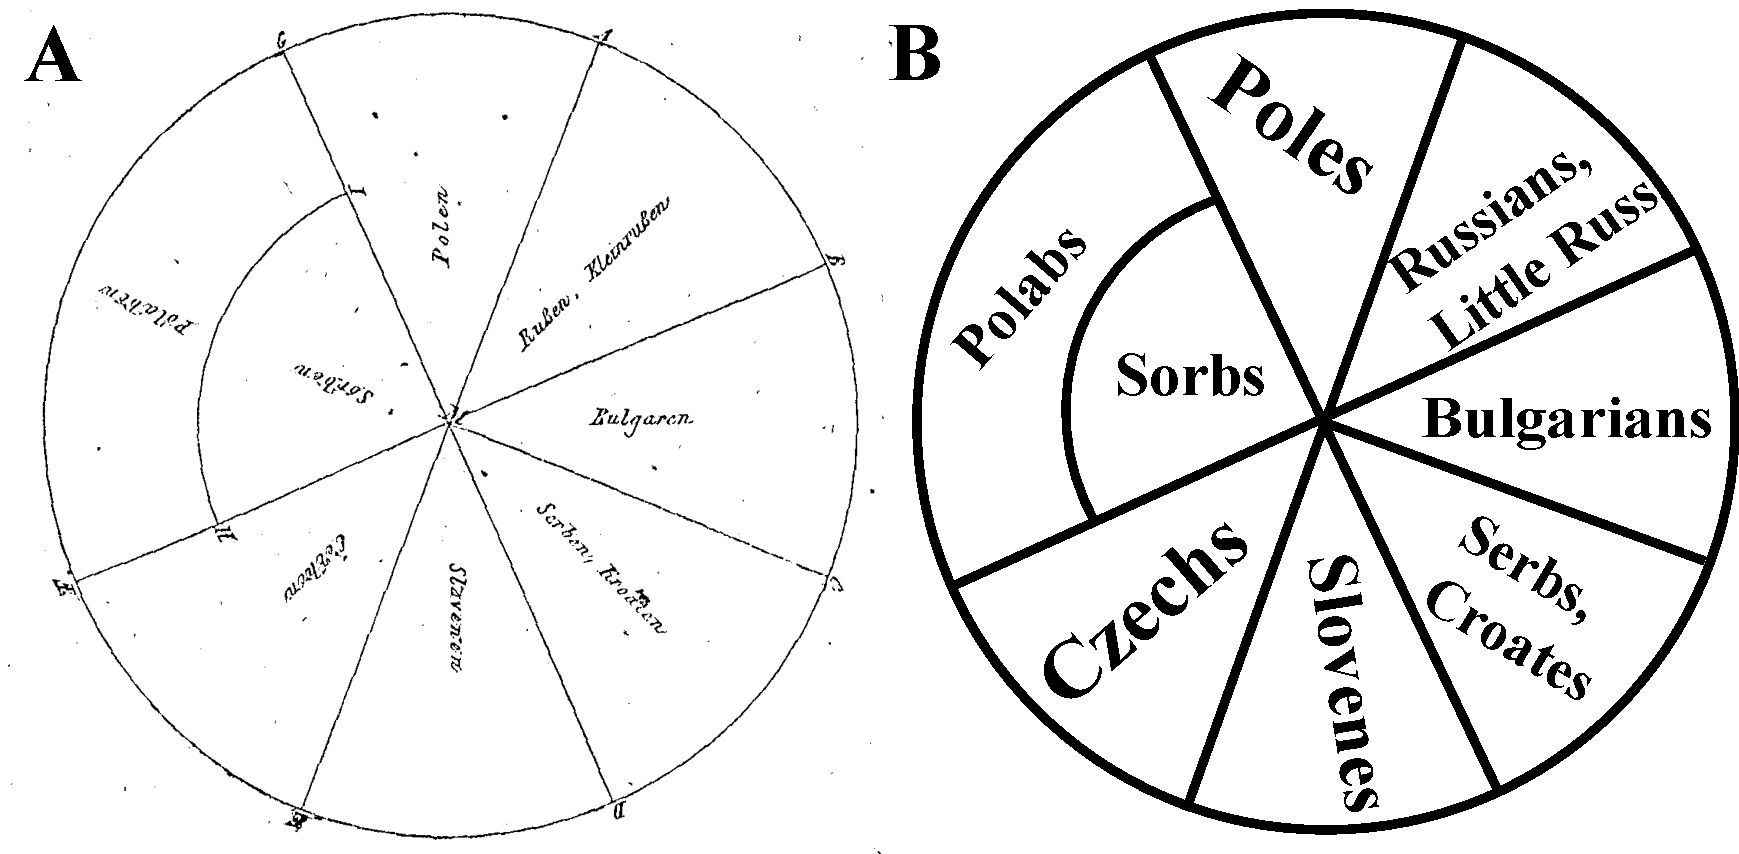
\includegraphics[width=0.75\textwidth]{images/schmidt-1875.pdf}
\caption{Schmidt's Wave Theory. A: Schmidt's visualization of the Wave Theory from 1875. B: English
translation.}
\label{fig:schmidt1875}
\end{figure}

\subsection{Early Arguments Against the Stammbaumtheorie}

\citet[118-120]{Geisler2013} distinguish three different kinds of
criticisms that have been raised against the family tree model (and in favor of the wave theory): (1)
practicability problems, (2) plausibility problems, and (3) adequacy problems. Practicability
problems refer to the problems in applying the tree model to analyse a given set of languages. 
Critics, such as \citet{Schmidt1872} mentioned above, point out in particular the issue of
conflicting evidence.
Plausibility problems refer to the realism of the family tree model and
are reflected in obvious simplifications provoked by the tree model. They are reflected in critics
emphasizing that languages do not necessarily split abruptly but slowly diverge accompanied by
complex waves of diffusion \citep{Schuchardt1870,Schmidt1872}. 
Adequacy refers to the purpose of
writing language history in historical linguistics. Critics complain that family trees break down
all vivid aspects that are substantial for the diversification of a language family to processes of
vertical descent. A similar argument has been brought up in biology, where the \emph{tree of life}
has been labeled the \emph{tree of one percent} given the fact that only a minimal amount of the
data seems to point to vertical descent \citep{Dagan2006}.
 
\citet{Geisler2013} emphasize that while all three types of criticism have been brought up against
the family tree model, it is clear their their theoretical strength differs. Refusing a model for
reasons of practicability is straightforward, but it cannot be used to prove that a model is wrong or
inadequate.  An inability to find evidence for a tree in a given dataset is no proof that the
family tree model is wrong, in the same way as the inability to distinguish borrowed from inherited
traits (especially in deeper time depths) can be considered proof against the existence of
tree-like divergence of languages.  \citet{Geisler2013} conclude, that stronger arguments against
the family tree model are those that challenge its plausibility, with respect to the presumed
split-process by which languages diverge, or its adequacy, with respect to its ability to provide a
full picture of language history in all its complexity.
 
Putting adequacy to the side, the distinction between practicability and plausibility can be redrawn
as a distinction between \emph{methodological} and \emph{theoretical} problems of the
Stammbaumtheorie. The former question the \emph{methodological possibility} to infer language trees
from linguistic data (referring to the power of the methods available to us), and the latter
question the adequacy of the model itself. While Schmidt's arguments were largely methodological in
nature, pointing to conflicts in the data (which are mostly based on a misunderstanding of the
nature of scientific inference and phylogenetic reconstruction, as pointed out in detail in
\citealt{Geisler2013}), Schuchardt's arguments are theoretical. He questions the process of
divergence itself, claiming that languages do not split in an abrupt, binary fashion, but rather
slowly diverge, while at the same time exchanging material in a non-vertical manner. An even greater
problem, not addressed in \citet{Schuchardt1870} is the possibility of \emph{convergence}. When
leading to \emph{hybridization}, it clearly contradicts the tree model in its core (see Section
\ref{sec:limits}), as trees can be
mathematically defined as directed, connected graphs in which all nodes only have one parent.
Interestingly, Schleicher was well aware of these problematic theoretical aspects of the tree model. He was explicitly pointing to the possibility of hybridization 
\citep{Schleicher1848} and he emphasized the often gradient transition underlying language
divergence \citep[21]{Schleicher1863}.
On the other hand, he deliberately ignored these aspects in the family
tree model, giving a strict preference to divergence and vertical inheritance.\footnote{Yet he may have tried to visualize genetic closeness
independently of elapsed time since separation, as can be seen from the tree in
\citet[7]{Schleicher1861}, where he notes that the length of the lines indicated the divergence
time, while the distance between the lines the degree of genetic closeness (`{Die länge der linien
deutet die zeitdauer an, die entfernung derselben von einander den verwantschaftsgrad.}'). This
can be interpreted in such a way that Schleicher tried to include potential convergence after
separation into his trees.}
 
Proponents of the
wave theory, on the other hand, were much less clear about the different processes they sought to
model. Do wave-like processes of language change reflect borrowing among closely related languages,
or are they intended to reflect language change in general? While \citet{Schuchardt1870} seems to distinguish
the two, pointing to \emph{horizontal lines} (`{horizontale Linien}') that make a network out of a
tree, \citet{Schmidt1872} is much less explicit, although he often invokes the idea of gradual
transitions between language borders \citep[200]{Schmidt1875}, thus emphasizing the gradualness of
diversification rather than the interference of vertical and lateral processes in language change.
Given the diversity of opinions and the lack of concreteness, it is
difficult to determine a core theory to which scholars refer when mentioning the Wave theory, and
while some see the wave theory as the horizontal counterpart of the family tree \citep[74]{Baxter2006a},
others see the wave theory as a theory explaining linguistic divergence
\citep[188-191]{Campbell1999}.

\section{The New Debate on Trees and Waves}
Along with the ``quantitative turn" in historical linguistics in the beginning of the 21st century
\citep[209f]{List2014d}, the debate on trees and waves has been recently revived. While most textbooks had
treated both models as a complementary view on \emph{external language history}\footnote{External
language history is here used in the sense of \citet[179-290]{Gabelentz1891} who distinguishes it from
internal language history pointing to different stages of one and the same language.}
\citep{Lehmann1992,Anttila1972} or as treating two completely different aspects of language change
\citep{Campbell1999}, more and more linguists now  discuss the models as opposing perspectives
\citep{Heggarty2010,Francois2014}. One reason for the revival of the discussion can certainly be
found in the prevalence of trees in recent phylogenetic studies in historical linguistics
\citep{Gray2003,Atkinson2006,Ringe2002,Pagel2009}. While both trees and waves had been playing a less
prominent role for a long time,\footnote{Even Morris Swadesh never used his lexicostatistic method
to produce family trees. Instead, he published a map on ``interrelationships of American Indian
languages'' that comes closer to an interpretation in terms of the wave theory
\citep[23]{Swadesh1959}.} biological methods for phylogenetic reconstruction applied to large
linguistic datasets now offer a much more transparent way to analyse and display large amounts of
language data in a tree diagram than the classical method of identifying shared innovations.
 
Yet not long after the first biological software packages were used for phylogenetic tree
reconstruction in linguistics, new
visualization techniques for \emph{splits networks} (most of them based on the NeighborNet algorithm,
\citealt{Bryant2004}), as provided by the SplitsTree software package \citep{Huson1998}, offered
scholars a fresh view on conflicts in their data. Often propagated as a reconciliation of
tree and wave theory \citep{Hamed2006,McMahon2005}, and easy to apply to
linguistic distance data, splits networks have quickly become a very popular tool in historical
linguistics \citep{Heggarty2010,Hamed2005,Bowern2010}.


\subsection{Phylogenetic Tree Reconstruction after the Quantitative Turn}
Classical phylogenetic tree reconstruction in historical linguistics is very similar to the basic
ideas of cladistics in biology (\citealt{Hennig1950}, see also \citealt[105-171]{Lass1997}), in so
far as it makes use of a small set of characters which are inherently weighted and represent \emph{unique
innovations} in order to uncover the phylogeny of a language family. The idea of unique innovations,
that is, changes that define a subgroup, is very old in linguistics, and can be found already in the
work of Karl Brugman (1849-1919), although it was later scholars like Isidore Dyen who
popularized the principle in historical linguistics (see \citealt{Chretien1963} and
\citealt{Dyen1953}). Brugmann himself justified the use of shared innovations in subgrouping as
follows:
\begin{quote}
  \small The only thing that can shed light on the relation among the individual language branches [...] are the
  specific correspondences between two or more of them, the innovations, by which each time certain
  language branches have advanced in comparison with other branches in their
  development. \cite[24]{Brugmann1967}\footnote{Our translation, original text: `Das einzige nun, was auf das Verhältnis der
  einzelnen Sprachzweige zu einander[, auf die Art des Hervorgangs der Einzelsprachen aus der idg.
  Ursprache] Licht werfen kann, sind die besonderen Übereinstimmungen zwischen je zwei oder mehreren
  von ihnen, die Neuerungen, durch die jedesmal gewisse Sprachzweige gegenüber den andern in der
  Entwicklung vorangeschritten erscheinen.'}
\end{quote}
The reason why linguists put such a great emphasis on shared innovations in subgrouping is obvious:
While related languages can easily share features they have retained from their common ancestor,
features which separate them from other languages in the same family and which may be interpreted as
a
new development can provide a strong argument for subgrouping. The problem, which is often
downplayed in this context, however, is how to \emph{identify} these \emph{exclusively shared
innovations}. If languages share common features (\emph{apomorphies} in cladistic terminology),
this does not necessarily mean that these features qualify as \emph{innovations}
(\emph{synapomorphies}), since they could have likewise (a)~been borrowed (see Section
\ref{sec:borrowing}) , (b)~been retained from th,e
common ancestor of all languages (\emph{symplesiomorphies}), (c)~been independently emerged
(\emph{homoplasies}), or (d)~been erroneously annotated as \emph{shared features}. Furthermore,
\emph{differential loss} or further development of features in subgroups may easily mask shared
innovations, and an innovation which was originally shared by a group of languages may give the
impression to be patchily distributed. This is further complicated by the fact that variation of
linguistic features occurs in all languages and may as well be traced back to the ancestral
language. If this is the case, and variation is later resolved randomly across the lineages, what
looks like a shared innovation would in fact rather represent a shared retention or an independent
development, thus, a combination of (b) and (c), as will be further discussed in Section
\ref{sec:ils}. None of these problems is new to historical linguistics, and we can find all of these
points, apart from the problem of variation in the proto-language, already in \citet{Brugmann1884},
who concludes that in order to be
applicable to subgrouping, proposed innovations must be \emph{frequent} enough to reduce the
possibility of chance (see also \citealt{Dyen1953}). 
 
How frequency is defined in concrete in historical linguistics is difficult to say, as scholars
often intuitively weight characters, assigning more importance to certain kinds of evidence (for
example form similarities in morphological paradigms, see \citealt{Nichols1996}) than to other types
(isolated lexical items, or frequent sound change patterns which are likely to recur independently),
and most debates regarding subgrouping center around the question of how the different types of
evidence should be weighted or the data interpreted \citep{Sagart2015}.  Phylogenetic approaches which were originally
developed for application in evolutionary biology offer a different approach to the problem by using
a larger pool of characters and explicit models of character evolution to automatically find the
phylogenetic tree that explains the data according to different criteria (probability, parsimony)
while at the same time determining which characters have been retained and which have been innovated
\citep{Greenhill2012}. 

\subsection{Linguistic Data and Data-Display Networks}
What many scholars misunderstand, however, is
that splits networks are a mere tool for data display \citep{Morrison2010} not a tool that directly
produces a phylogenetic analysis. While splits
networks are very useful for exploratory data analysis, notably, 
\begin{quote}
(1) the automatic extraction of previously unknown patterns with regard to groups of
objects, without using known structures in the data;
(2) the detection of anomalous objects in the dataset;
and (3) providing a compact representation of the
dataset, which can be easily visualized as a connected
graph \citep[2]{Morrison2014b},
\end{quote}
they do not produce any hypothesis on how languages or biological species diverged, and they must be
strictly distinguished from explicit \emph{evolutionary networks}, displaying `{evolutionary
relationships between ancestors and descendants' \citep[43]{Morrison2011}.
\textcolor{red}{develop this part a bit further, maybe half a page, using quotes from morrison or
the like, also being fair, regarding the usefulness of data-display networks}
\subsection{Shared Innovations and Historical Glottometry}
\textcolor{red}{develop further, thereby making explicitly clear that historical glottometry does
confuse the idea of shared innovations in historical linguistics, since it ignores homoplasy,
differential loss, and polarity of change}
 
A very recent approach which also attempts to dismiss the tree model is the theory of
\emph{historical glottometry} \citep{Francois2014,Kalyan2016}. Similar to the arguments brought up
by \citet{Schmidt1872}, glottometry results from the dissatisfaction of conflicting data in
historical linguistics.  Furthermore, glottometry follows \citet{Ross1988} in assuming that language
divergence may proceed in form of concrete \emph{separation} (\emph{social split} according to
\citealt{Francois2014}) and \emph{dialect divergence}. While the former process involves the
complete separation of the speakers of a given language, mostly based on geographic dislocation of
parts of a population, the latter involves the slow divergence of language varieties into dialect
areas which may later result in a complete split and the loss of mutual intelligibility.
Essentially, this argument comes close to the one of \citet{Schuchardt1870}, as it attacks the
process of concrete language split as it is visually suggested by the tree model. Given the high
diffusability of linguistic features across mutually intelligible varieties, a fully resolved tree
reconstruction showing language divergence in split processes may become difficult if not impossible
in such a scenario of language divergence. \citet{Ross1988} uses the term ``linkage" to refer to
closely related language varieties that diffused rather than separated and uses specifically marked
multifurcating nodes to highlight them in his genetic subgrouping of Oceanic languages.
\citet{Kalyan2016} criticize this solution as unsatisfying, lacking not only scientific rigor due
to the displayed uncertainty of divergence, but also ignoring the fact that innovations can easily
spread across dialect networks, thus creating intersecting, fuzzy subgroups. The solution proposed
by historical glottometry is to use the classical comparative method to collect shared innovations
for the language family under investigation, and to display the innovations as weighted isogloss
maps in which weighting is represented by the thickness of a given isogloss. This is illustrated in
Figure \ref{fig:glotto}A, where four hypothetical languages are given which are connected by three
isoglosses of which two are in conflict with each other.

\begin{figure}[htb]
  \centering
  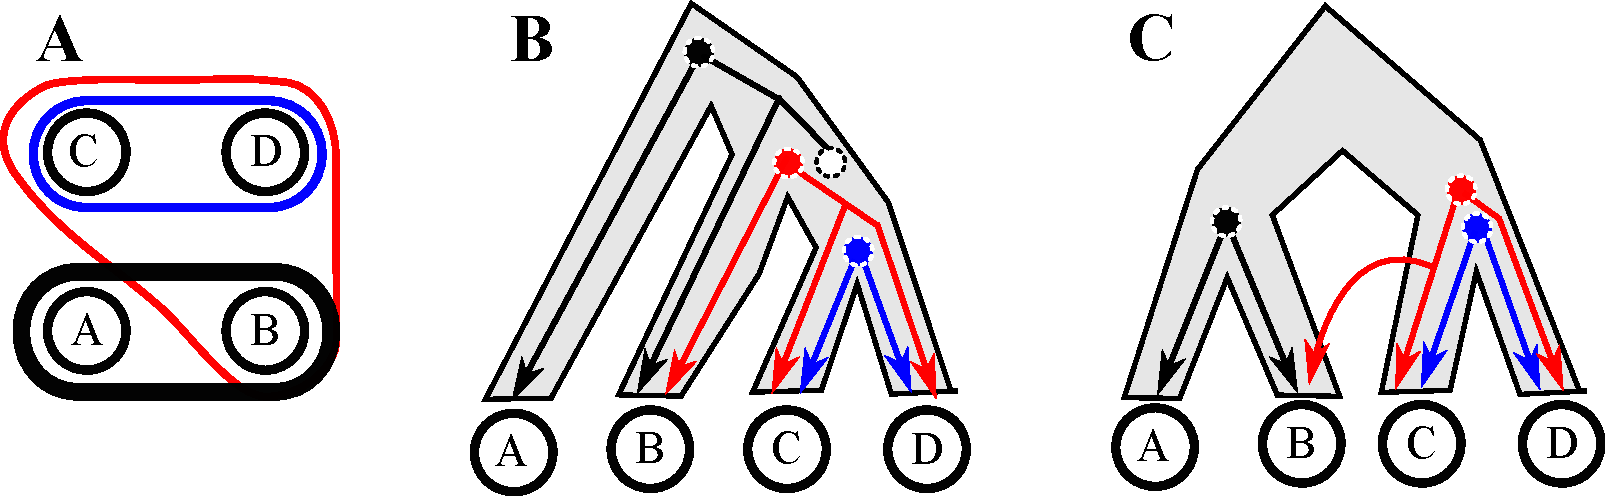
\includegraphics[width=1\textwidth]{images/glottometrie.pdf}
  \caption{Historical glottometry, the family tree model, and an evolutionary network. A shows a glottometric diagram showing
  weighted isoglosses drawn between languages sharing an innovation which are in apparent conflict
  with each other. B shows how the same scenario can be explained with help of a family tree by
  assuming differential loss of the black isogloss. C shows an evolutionary network representing
  another possible explanation for the patterns by assuming that the red innovation was borrowed
  from language C into language B.}
  \label{fig:glotto}
\end{figure}
 

Three general problems of the method of historical glottometry can be mentioned in this context:
First, the resulting visualizations can by no means qualify as phylogenetic analyses, as they lack
the time dimension. They are more similar to data display networks, and the fact that the isogloss
strength is aggregated in a simple number makes them not much more informative then splits networks
produced with the NeighborNet algorithm. This does not mean that the measure proposed by
glottometry do not have their specific value, but unlike the tree model which displays a concrete
evolutionary hypothesis, glottometric diagrams are mere tools for data visualization.\footnote{Mathematically, the isogloss model proposed by glottometry
corresponds to a \emph{hypergraph}, in which edges can connect more than one vertex
\citep[122f]{Newman2010}. Given that hypergraphs are equivalent to \emph{bipartite networks}, it also seems
that with the existing metrics applied in glottometry, not all mathematical possibilities are
exhausted, and instead of weighting isoglosses using the \emph{cohesiveness} value proposed in
\citep{Francois2014}, it might be interesting to look into different \emph{projections} of bipartite into
monopartite graphs \citep[124f]{Newman2010}.}
 
Second, the assumption that the tree
model can be falsified if true synapomorphies (shared innovations) can be found which are in
conflict with any possible family tree topology is logically problematic.
Shared innovations in the true cladistic sense are
never in conflict with a tree, since they are \emph{defined} as those elements which constitute the
tree. They are rigorously distinguished from shared retentions, lateral transfer, and
parallel developments \citep{Fleischhauer2009}.\footnote{The problem of \emph{shared innovations}
often leads to confusion in linguistics, as the term itself is explanative, while scholars often use
it descriptively. The descriptive use of explanative terminology can be seen as a general problem in
linguistic terminology, as reflected in terms like `{pronominalization}' (see
\citealt[2]{Jacques2016c}), or `{polysemy}' (see \citealt{Francois2008},
\citealt{List2013a}), or `{assimilation}' (see \citealt[32]{List2014d}).}
A cladistic analysis seeks to identify which
of a large pool of \emph{possible characters} could qualify to define a subgroup and thus reflect
\emph{potentially} true shared innovations. If a supposed set of innovations shows internal conflict
with possible tree topologies, this means, from a cladistic perspective, that some of these
innovations have been wrongly proposed. This is illustrated in Figure \ref{fig:glotto}B, where the data from Figure
\ref{fig:glotto}A is explained by differential loss of a shared character in one clade of a tree. Given
that we can often hardly distinguish whether homologous characters in languages are due to independent
change or inheritance,\footnote{This is explicitly admitted by \citet{Francois2014} in the section
where he explains how the data was assembled.} conflicts with possible tree topologies
can by no means be taken as rigorous proof that a substantial
amount of the data cannot
be explained by a tree. 
 
Third, given that \citet{Kalyan2016} admit that innovations develop
\emph{somewhere}, their approach is by no means less agnostic than the use of multifurcating tree
topologies by \citet{Ross1988}, as we would assume that an innovation first occurs in a small
community from where it spreads. Theoretically, it may thus be possible to draw explicit pathways of
diffusion which could be rendered as horizontal edges in an evolutionary network, as illustrated in
Figure \ref{fig:glotto}C.
 

\section{Saving the Trees from the Critics}
Given the logical necessity to allow for divergence, a specific part of language history can be
modeled with help of a tree if specific processes like recombination (hybridization, creolization)
can be excluded. That such a tree model does not necessarily represent all aspects of language
history is obvious, and even the strongest tree proponents would not deny it. Whether the amount
of inheritance versus borrowing in language history is as low as it was supposed for biology, where
tree critics have labeled the tree of life as the ``tree of one percent'' \citep{Dagan2006} is an
interesting question worth being pursued further. However, given that we know that language varieties can
diverge to such an extent that they lose mutual intelligibility \emph{necessitates} a model for
language history which handles divergence and splits of lineages. How these splits proceed in the
end, whether they are best viewed as multifurcations after the split of a larger dialect continuum
in several parts, or as bifurcations, depends on our insights into the language family under
investigation and into the processes of external language change in general.  
 
When scholars point out that a given dataset lacks tree-like signal, or that the tree-like signal
for the subgrouping of a given language family is not strong, they often take this as direct
evidence for large-scale language contact or linkage scenarios \citep{Ross1988}.  This, however, is
by no means the only explanation for reticulations in datasets, and there are many other reasons why a given
data selection may fail to reveal a tree (see the general overview in
\citealt[44-66]{Morrison2011}). The most obvious and in cases of large dataset most frequent reason
are erroneous codings which occur especially in those cases where the data has not been thoroughly
checked by experts in the field \citep{Geisler2010}, or where automatic analyses have introduced
a strong bias. Another obvious reason for reticulation in a dataset is the selection of the data. Commonalities in sound change
patterns and grammatical features, for example, often do not represent true shared innovations but independent development, and especially for sound changes it is often very hard to distinguish between synapomorphy and homoplasy \citep[182f]{Chacon2015a}, which is exacerbated by the fact that
the majority of sound change patterns are extremely common, while rare sound changes are often very difficult to prove. 
 

Apart from borrowing, dialect differentiation, data coding, and homoplasy,
another often overlooked cause of reticulations in the data is the process of \emph{incomplete
lineage sorting} \citep{Galtier2008}. Incomplete lineage sorting is a well-known process in
biology, during which polymorphisms in the ancestral lineages are inherited by the descendant
species when rapid divergence occurs \citep{Rogers2014}. Incomplete lineage sorting can explain 
why 30\% of the genes in a Gorilla's genome are more similar to the human genome or to the
Chimpanzee genome although human and chimpanzee are the closest relatives \citep{Scally2012}. 
In a recent study, \citet{List2016h} proposed that incomplete lineage sorting may likewise occur in
language history, given  
the multiple sources of polymorphisms in language change, ranging from near synonymy of lexical
items via suppletive paradigms to word derivation.
 
Apart from these language-internal factors of polymorphisms which may be inherited across lineages,
before they are later randomly resolved, a further factor not mentioned by \citet{List2016h} is
\emph{variation in the population of speakers}, or \emph{sociolinguistic variation}, which may even occur in one and the
same speaker.  The process of incomplete lineage sorting is further illustrated in Figure
\ref{fig:ils}, where the two aspects, namely sociolinguistic variation, and language-internal
variation are contrasted. Note that in neither of the cases we even need to invoke neither strong
language contact nor situations of large scale diffusion in dialect networks. Both patterns are
perfectly compatible with a ``social split" situation as invoked by \citet{Francois2014}, although
they are based on fully resolved bifurcating trees. This shows that supposed reticulations in the
data, or lack of tree-like signal in the data do not necessarily prove the absence of tree-like
patterns of divergence. They rather expose the weakness of our methods to find the tree in the
forest of individual histories of linguistic traits. In the following, we will illustrate this
in more detail by showing how variation \emph{inherited} from the ancestor language may be lost
incompletely across lineages, and by showing how the failure to identify \emph{true} innovations may
lead us astray when searching for convincing phylogenies.

\begin{figure}[htb]
  \centering
  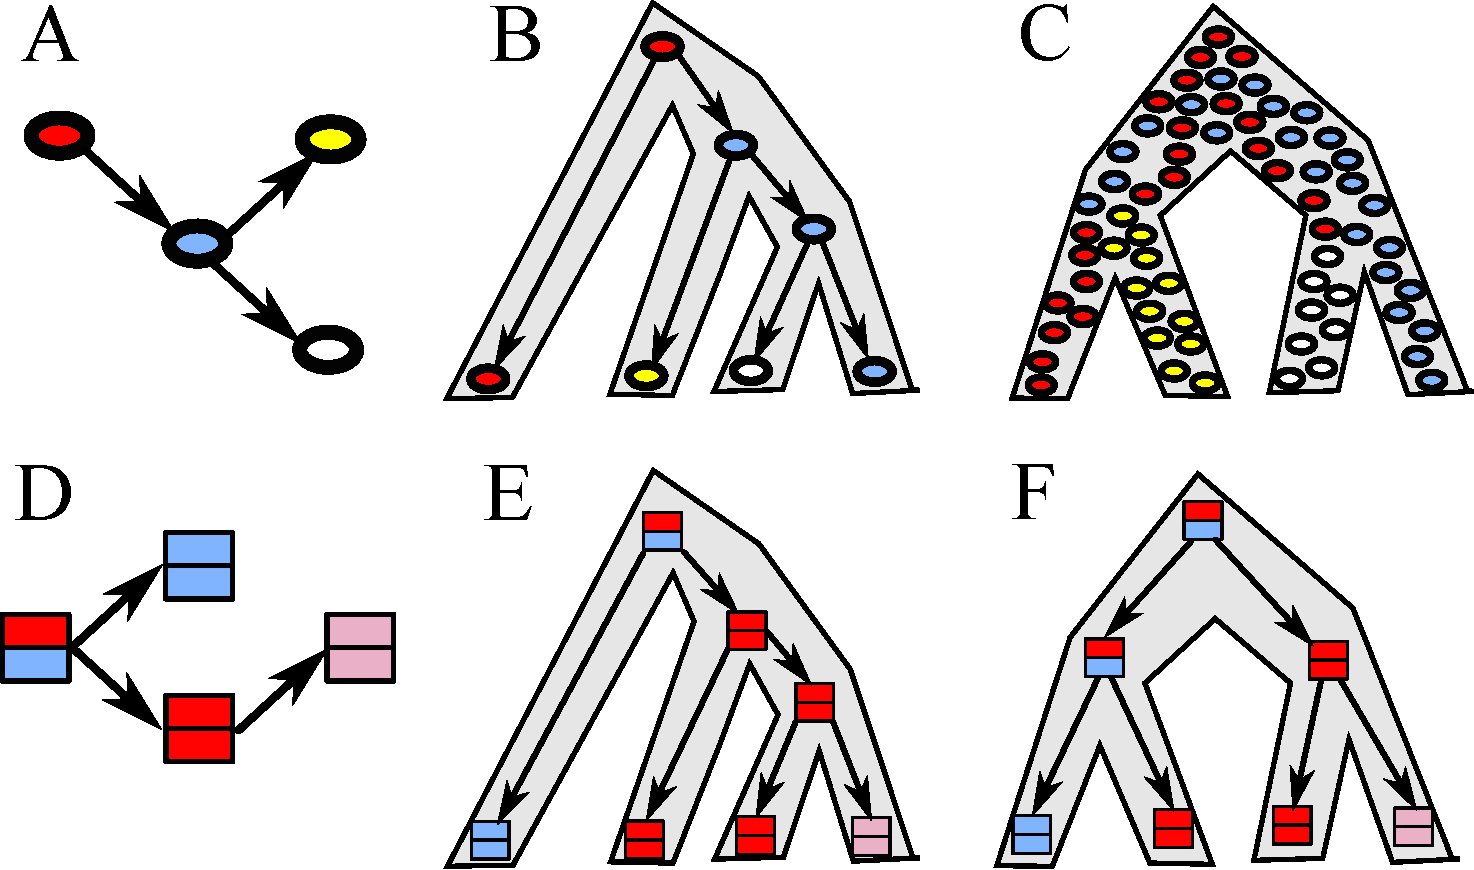
\includegraphics[width=\textwidth]{images/ils.pdf}
  \caption{Incomplete lineage sorting due to sociolinguistic (A-C) and linguistic variation (D-F) and its impact   on phylogenetic reconstruction and genetic subgrouping. A shows a pattern of known directional   evolution of a character (e.g., a sound change pattern), and B shows one of the most parsimonious
  trees resulting from the pattern. C shows an alternative pattern by assuming that the blue   character already evolved in the ancestral language where it was used as a variant along with the original red character. Since the variation already occurred at the time of the ancestral languages, it was inherited in the two descendant languages from which the character further developed. As a result, another tree topology can be reconstructed. D gives an example for a process of paradigm leveling, and E and F show two possible equally parsimonious scenarios invoking different tree topologies each.}
  \label{fig:ils}
\end{figure}

\subsection{The Benefit of Trees in Language Comparison}
\textcolor{red}{Write briefly about the benefit of trees: they give us polarity where we don't find
it when we lack information on polarity of processes, they give us rates, thus allowing us to access
how easy things can happen, and they give us history, as they allow to propose ancestral nodes.}
\textcolor{green}{Rates and trees: If we are dealing with phenomena like sound change, or semantic
change, we want to know the degree of paralellism, to which they could occur independently. If we
deny any splits in language history and any internal topology of splits in language families, we
will necessarily count all changes only once, thus largely underestimating the potential degree of
parallel change, bring tukano language example}

\subsection{Inherited Variation and Incomplete Lineage Sorting}\label{sec:ils}
\textit{Lexically-specific sound changes} play an important role in historical glottometry, based on
the assumption that
they are ``strongly indicative of genealogy, because they are unlikely to diffuse across separate
languages'' \citet[178]{Francois2014}. Out of 474 shared traits which are classified as innovations in \citet{Francois2014}, 116 (24\%) belong to this type. In view of the low
diffusibility of such traits,\footnote{This assertion remains to be demonstrated, but we
accept it for the sake of argument.} overlapping isoglosses constitute a major problem
for the tree model in the view of glottometry. Regardless of whether lexically-specific sound changes have more difficulty to
cross language boundaries than other types of features, overlapping innovations can, as mentioned
above, also be accounted for by assuming the existence of variation in the
proto-language.\footnote{In this case, however, we can no longer speak of true innovations in the cladistic
sense, as, as mentioned above, the term innovation is explanative and not descriptive, and
presupposes that a trait is uniquely shared by the subgroup which it defines.}

Languages are never completely uniform, and fieldwork linguists working on unwritten languages
commonly notice that even siblings may present significant differences in the pronunciation of
certain words or even morphological paradigms (see for instance \citealt[29-30]{genetti07grammar}).
While some innovations can spread quickly to the entire community (or at least to all members of a
specific age-group), in other cases it is possible for two competing forms (innovative vs archaic)
to remain used in the same  speech community for a considerable period of time. This is observed in
particular with sporadic changes, such as irregular metatheses, dissimilation, assimilation, or
item-specific analogy.

When language differentiation occurs while forms are still competing, daughter languages can inherit
the competing forms; then the innovative form may eventually prevail or disappear in a
non-predictable way in each daughter language. If such a situation occurs, the distribution of the
innovation will not be relatable to the phylogenetic tree.  This phenomenon is better illustrated by
analogical levelling rather than by sporadic sound changes, as in the case of the former the
variation comes from well-understood morphological alternations that have been generalized in
different ways in different language varieties, though the same account  would be valid of the
sporadic changes.
 
To illustrate how alternation and variation in the proto-language can blur the phylogeny, we take the example of the reflexes of proto-Germanic *\ipa{knabō, knappaz} `boy' (Figure \ref{fig:knabe}),\footnote{The reflexes of this proto-form have developped distinct meanings in the attested languages, including `squire', but this aspect is not considered here.} an n-stem noun whose reflexes in the modern and ancient languages are particularly complex (data from \citealt[71,128]{kroonen11nstems}, \citealt[294]{kroonen13dict}).
From the attested ancient and modern forms (if the known sound laws are applied backwards), no fewer than four protoforms have to be postulated:  \ipa{*knaban-}, \ipa{*knapan-}, \ipa{*knabban-} and \ipa{*knappan-}. Some languages have more than one reflex of this etymon (with diverging specialized meanings), and their distribution does not fit any accepted classification of the Germanic languages: for instance, while nearly all Germanicists agree on the existence of an Anglo-Frisian `Ingvaeonic' branch, we see that English sides with either German (in having a reflex of \ipa{*knaban-}) or with Dutch (the Old English reflex of \ipa{*knapan-}, lost in modern English) rather than Frisian.

   \begin{figure}[h]
   \caption{Several layers of variation: The etymon *\ipa{knabō, knappaz} `boy' in Germanic.} \label{fig:knabe}   \centering
  \begin{tikzpicture}
  \node (A) at (0,5) {(0) \ipa{*gnóbʰ-ōn, gnobʰ-nós}};
   \node (B) at (0,3) {(1) \ipa{*knabō, knappaz}};
   \node (C) at (-3,1) {(2a) \ipa{*knabō, knabbaz}};
   \node (D) at (3,1) {(2b) \ipa{*knapō, knappaz}};
   \node (E) at (-5,-1) {(3a) \ipa{*knaban-}};
   \node (F) at (-2.5,-1) {(3a') \ipa{*knabban-}};
   \node (G) at (2,-1) {(3b) \ipa{*knapan-}};
   \node (H) at (5,-1) {(3b') \ipa{*knappan-}};
   \node (I) at (-6,-3) {OE \ipa{cnafa-}, OHG \ipa{cnafa-}};
   \node (J) at (-2.5,-3) {OHG \ipa{knappo}};
   \node (K) at (2,-3) {OE \ipa{cnapa-}, OS \ipa{knapo-}, OD \ipa{knapo-}};
   \node (L) at (5.5,-4) {OFri. \ipa{knappa}};
   \node (M) at (-6,-5) {E \ipa{knave}, G \ipa{Knabe}};
   \node (N) at (-2.5,-5) {G \ipa{Knappe}};
   \node (O) at (2,-5) {D \ipa{Knaap}};
\tikzstyle{peutetre}=[->,dotted,very thick,>=latex]
\tikzstyle{sur}=[->,very thick,>=latex]
\draw[sur] (A)--(B);
\draw[peutetre] (B)--(C);
\draw[peutetre] (B)--(D);
\draw[peutetre] (C)--(E);
\draw[peutetre] (C)--(F);
\draw[peutetre] (D)--(G);
\draw[peutetre] (D)--(H);
\draw[sur] (E)--(I);
\draw[sur] (F)--(J);
\draw[sur] (G)--(K);
\draw[sur] (H)--(L);
\draw[sur] (I)--(M);
\draw[sur] (J)--(N);
\draw[sur] (K)--(O);
\end{tikzpicture}
\end{figure}

Unlike most other language families, the detailed knowledge that has accumulated on the history of Germanic languages allows to go further than stating the presence of irregular correspondences: it is possible to account for them with a detailed model. It is now near-universally accepted that doublets such as those are due to the effect of Kluge's law on the endings of n-stem nouns in pre-proto-Germanic (stage 0, \citealt{kluge1884dehnung, kroonen11nstems}). 

The paradigm of the noun `boy' (and all nouns of the same type) in proto-Germanic  (stage 1) had an alternation between *\ipa{-b-} and *\ipa{-pp-}. This complex  alternation was variously levelled as *\ipa{-b-}/\ipa{-bb-} or *\ipa{-p-}/\ipa{-pp-} by stage 2; note that within a single language, not all items belonging to this declension class underwent levelling in the same way, and that some languages even have competing innovative (OE \ipa{cnapa}  from \ipa{*knapan-}) and archaic (OE \ipa{cnafa}  from \ipa{*knaban-}) forms for the same etymon (in this particular case, note that only the archaic form has been preserved, with a different meaning, in modern English \ipa{knave}).
After simplification of the *\ipa{-b-}/*\ipa{-pp-} alternation, all languages underwent a second wave of analogy, generalizing either the stem of the nominative (archaic \ipa{*knaban-} or innovative \ipa{*knapan-}) or that of the genitive (archaic \ipa{*knappan-} or innovative \ipa{*knabban-}), resulting in the four variants attested throughout Germanic languages.

We do not deny the potential value of item-specific changes of this type as evidence for studying phylogeny. However, it is obvious that isoglosses based on item-specific analogical levelling and sporadic sound change \emph{will overlap} with each other, since competing forms can be maintained within the same language variety and only later be incompletely sorted across different lineages.


\subsection{The Problem of Identifying Lexical Innovations}\label{sec:borrowing}
In order to identify inherited lexical innovations and distinguish them from recent borrowings, the
method of historical glottometry uses a fairly uncontroversial criterion: Etyma whose reflexes
follow regular sound correspondences are considered to be inherited \citep[176-8]{Francois2014}.
Thus, whenever a common proto-form can be postulated for a particular set of words across several
languages (which can thus be derived from this proto-form by the mechanical application of regular
sound changes), it is considered in this model to be part of the inherited vocabulary, and can be
used, if applicable, as a common innovation.

This approach however neglects an important factor: while regular sound correspondences is a necessary condition for analyzing forms in related languages as cognates, i.e. originating from the same etymon in their common ancestor,\footnote{Note however that cognacy is a more complex concept than is usually believed (\citealt{list16cognacy}), and that even forms originating from exactly the
same etymon in the proto-language may present irregular correspondences due to analogy.} it is not
a \textbf{sufficient} condition due to the existence of \textbf{undetectable borrowings} and
\textbf{nativized loanwords}.  



\subsubsection{Undetectable Borrowings}
Sound changes are not always informative enough to allow the researcher to discriminate between inherited word and borrowing. When a form contains phonemes that remained unchanged, or nearly unchanged, from the proto-language in all daughter languages (because no sound change, or only trivial changes, affected them), there is no way to know whether it was inherited from the proto-language or whether it was borrowed at a later stage. 

This type of situation is by no means exceptional, and can be found in various language families. We present here three examples of borrowings undetectable by phonology alone: `aluminum' in Tibetan languages, `pig' in some Algonquian languages, and `palace' in Semitic. 
Amdo Tibetan \ipa{hajaŋ} `aluminum' and Lhasa \ipa{hájã} `aluminum' look like they regularly originate from a Common Tibetan form *\ipa{ha.jaŋ}.\footnote{In Amdo Tibetan, Common Tibetan \ipa{h-}, \ipa{j-}, \ipa{-a} and \ipa{-aŋ} remain unchanged (\citealt{gong16amdo}). In Lhasa Tibetan, two sound changes relevant to this form occurred: a phonological high tone developped with the initial \ipa{h-}, and \ipa{-aŋ} became nasalized \ipa{ã}.} This is of course impossible for obvious historical reasons, as aluminum came into use in Tibetan areas in the twentieth century, at a time when Amdo Tibetan and Lhasa Tibetan were already completely unintelligible. This word is generally explained (Gong Xun, p.c.) as an abbreviated form of \ipa{ha.tɕaŋ jaŋ.po} `very light', but this etymology is not transparent to native speakers of either Amdo or Lhasa Tibetan. This word has been coined only once,\footnote{We are not aware of a detailed historical research on the history of this particular word, but in any case it matters little for our demonstration whether it was first coined in Central Tibetan or in Amdo.} and was then borrowed into other Tibetan languages\footnote{In some Tibetan languages such as Cone \ipa{hæ̀jãː}, \citet[306]{jacques14cone}, there is clear evidence that the word is borrowed from Amdo Tibetan and is not native (otherwise $\dagger$\ipa{hæ̀jaː} would have been expected). } and neighboring minority languages under Tibetan influence (as for instance Japhug \ipa{χajaŋ} `aluminum').
In this case a phonetic borrowing from Amdo \ipa{hajaŋ} could only yield Lhasa \ipa{hájã}, since \ipa{h-} only occurs in high tone in Lhasa, and since final \ipa{-ŋ} has been transphonologized as vowel nasality.\footnote{Likewise, in the case of borrowing from Lhasa into Amdo, the rhyme \ipa{-aŋ} would be the only reasonable match for Lhasa \ipa{-ã}.} 

Several Algonquian languages, share a word for `pig' (Fox \ipa{koohkooša}, Miami \ipa{koohkooša} and Cree \ipa{kôhkôs}) ultimately of Dutch origin (\citealt{goddard74dutch}, \citealt{costa13borrowing}). \citet[266]{hockett57k} pointed out that these forms must be considered to be loanwords `because of the clearly post-Columbian meaning; but if we did not have the extralinguistic information the agreement in shape (apart from M[enominee]) would lead us to reconstruct a [Proto-Central-Algonquian] prototype.' The forms from these three languages could be regularly derived from Proto-Algonquian *\ipa{koohkooša}, a reconstruction identical to the attested Fox and Miami forms.
%Ojibwe gookoosh

Semitic languages abound in common vocabulary which presents the same correspondences as inherited vocabulary, but which was diffused after the breakup of the family. For instance, from Biblical Hebrew \ipa{hêkāl} `palace' and Arabic \ipa{haykal} `palace', it would be possible to reconstruct a Proto-Semitic etymon *\ipa{haykal(u)}; it is however well-known that these words originate from Sumerian \ipa{é.gal} `palace', probably through Akkadian \ipa{ekallum}, and that borrowing from Akkadian took place at a time when the ancestors of Hebrew and Arabic respectively were already distinct languages.

Undetectable borrowings are also a pervasive phenomenon in Pama-Nyungan, where with a few exception such as the Arandic and Paman groups, most languages present too few phonological innovations to allow easy discrimination for loanwords from cognates (\citealt[46]{koch04method}).
The same situation can be observed even if latter sound changes apply to both borrowings and inherited words. Whenever borrowing takes place after the break-up of two languages, but before any diagnostic sound change occurred in either the donor or the receiver language, phonology alone is not a sufficient criterion to distinguish between inherited words and loanwords. 
 
A classical case is that of Persian borrowings in Armenian. As
\citet[16-17]{huebschmann97armenische} put it, `in isolated cases, the Iranian and the genuine
Armenian forms match each other phonetically, and the question whether borrowing [or common
inheritance] has to be assumed must be decided from a non-linguistic point of view.'\footnote{Our
translation, original text: `In einzelnen Fällen kann allerdings das persische und echt armenische Wort sich lautlich decken und die Frage, ob Entlehnung anzunehmen ist oder nicht, muss dann nach andern als sprachlichen Gesichtspunkten entschieden werden.'} Table \ref{tab:armenian} presents a non-exhaustive list of such words.
 
\begin{table}[h]
\caption{Armenian words which cannot be conclusively demonstrated to be either borrowings from Iranian or inherited words from a phonetic point of view    } \centering \label{tab:armenian}
\begin{tabular}{lllllll}
\toprule 
Armenian & Meaning & Indo-Iranian & Reference \\
\midrule 
\ipa{naw}& boat & Skt. \ipa{nau-} & \citet[16-17;201]{huebschmann97armenische},\\
&&& \citet[466;715]{martirosyan10etymological} \\
\midrule 
\ipa{mēg}& mist & Skt. \ipa{megha-},  & \citet[474]{huebschmann97armenische},\\
&&Avestan \ipa{maēɣa-}& \citet[466;715]{martirosyan10etymological} \\
\midrule 
\ipa{mēz}& urine & Skt. \ipa{meha-} & \citet[474]{huebschmann97armenische},\\
&&& \citet[466;715]{martirosyan10etymological} \\
\midrule 
\ipa{sar}& head & Skt. \ipa{śiras-} & \citet[236;489]{huebschmann97armenische},\\
&&Y.Avestan \ipa{sarah-}& \citet[571]{martirosyan10etymological} \\
\midrule 
\ipa{ayrem}& burn & Skt. \ipa{edh-} & \citet[418]{huebschmann97armenische},\\
&&& \citet[145]{martzloff16geri} \\
\bottomrule
\end{tabular}
\end{table}
 
The Armenian case shows that undetectable loans are not restricted to cases like those studied above, when a particular word only contains segments which have not been affected by sound changes from the proto-language to all its daughter languages. Undetectable loans are possible when a particular word is borrowed before any sound change which could affect its phonetic material occurred in either the giver or recipient language, even if numerous sound changes occurred \textit{after} borrowing took place. It is possible that post-borrowing sound changes may even remove phonetic clues which could have allowed to distinguish between loanwords and inherited words.

What has been illustrated above can be seen as clear evidence that undetectable borrowings can occur
even when two language varieties are mutually unintelligible. Neglecting the distinction between
inherited words and undetectable borrowings, as in the approach propagated in historical glottometry, amounts to losing crucial
historical information, and it does not seem justified to blame the family tree model for an insufficiency
of our linguistic reconstruction methodology.

\subsubsection{Nativization of Loanwords}
In the previous section, we discussed cases when borrowing took place before diagnostic sound changes, thus making it impossible to effectively use sound changes to distinguish between loanwords and inherited words. There is however evidence that even when diagnostic sound changes exist, they may not always be an absolutely reliable criterion.

When a particular language contains a sizeable layer of borrowings from another language, bilingual speakers can develop an intuition of the phonological correspondences between the two languages, and apply these correspondences to newly borrowed words, a phenomenon known as loan nativization.

The best documented case of loan nativization is that between Saami and Finnish (the following discussion is based on \citealt{aikio06nativization}). Finnish and Saami are only remotely related within the Finno-Ugric branch of Uralic, but  Saami has borrowed a considerable quantity of vocabulary from Finnish, some at a stage before most characteristic sound changes had taken place, other more recently. Table \ref{tab:native} presents examples of cognates between Finnish and Northern Saami illustrating some recurrent vowel and consonant correspondences.

\begin{table}[h]
\caption{Examples of sound correspondences in inherited words between Finnish and Northern Saami (data from \citealt[27]{aikio06nativization})} \centering \label{tab:native}
\begin{tabular}{lllll}
\toprule
Finnish & Northern Saami & Proto-Finno-Ugric & Meaning \\
\midrule
\ipa{käsi} & \ipa{giehta} & *\ipa{käti} & `hand' \\
\ipa{nimi} & \ipa{namma} & *\ipa{nimi} & `name' \\
\ipa{kala} & \ipa{guolli} & *\ipa{kala} & `fish' \\
\ipa{muna} & \ipa{monni} & *\ipa{muna} & `egg' \\
\bottomrule
\end{tabular}
\end{table}

The correspondence of final \ipa{-a} to \ipa{-i} and final \ipa{-i} to \ipa{-a} in disyllabic words found in the native vocabulary, as illustrated by the data in Table \ref{tab:native}, is also observed in Saami words borrowed from Finnish, including recent borrowings, such as \ipa{mearka} from \ipa{merkki} `sign, mark' and \ipa{báhppa} from \ipa{pappi} `priest' (from Common Slavic *\ipa{păpъ}, itself of Greek origin), even though the sound change from proto-Uralic to Saami leading to the correspondence \ipa{-a} : \ipa{-i} had already taken place at the time of contact. These correspondences are pervasive even in the most recent borrowings, to the extent that according to \citet[36]{aikio06nativization} `examples of phonetically unmarked substitutions of the type F[innish] \ipa{-i} > Saa[mi] \ipa{-i} and F[innish] \ipa{-a} > Saa[mi] \ipa{-a} are practically nonexistent, young borrowings included.'

In cases such as \ipa{báhppa} `priest', the vowel correspondence in the first syllable \ipa{á} : \ipa{a} betrays its origin as a loanword, as the expected correspondence for a native word would be \ipa{uo} : \ipa{a} as in the word `fish' in Table \ref{tab:native} (\citealt[35]{aikio06nativization} notes that this correspondence is never found in borrowed words).

However, there are cases where recent loanwords from Finnish in Saami present correspondences indistinguishable from those of the inherited lexicon, as \ipa{barta} `cabin' from Finnish \ipa{pirtti}, itself from dialectal Russian \ipa{перть} `a type of cabin', which show the same \ipa{CiCi} : \ipa{CaCa} vowel correspondence as the word `name' in table \ref{tab:native}. Here again, the foreign origin of this word is a clear indication that \ipa{barta} `cabin' cannot have undergone the series of regular sound changes leading from proto-Finno-Ugric *\ipa{CiCi} to Saami \ipa{CaCa}, and that instead the common vowel correspondence \ipa{CiCi} : \ipa{CaCa} was applied to Finnish \ipa{pirtti}.
 
Loan nativization can also occur between genetically unrelated languages. A clear example is provided by the case of Basque and Spanish (\citealt[53-54]{trask00chronology}, \citealt[21-3]{aikio06nativization}). 
A recurrent correspondence between Spanish and Basque is word-final \ipa{-ón} to \ipa{-oi}. Early Romance *\ipa{-one} (from Latin \ipa{-onem}) yields Spanish \ipa{-ón}. In Early Romance borrowings into Basque, however, this ending undergoes the regular loss of intervocalic *\ipa{-n-} (a Basque-internal sound change), and yields *\ipa{-one} $\rightarrow$ *\ipa{-oe} $\rightarrow$ \ipa{-oi}. An example of this correspondence is provided by Spanish \ipa{razón} and Basque \ipa{arrazoi} `reason' both from Early Romance *\ipa{ratsone} (from the Latin accusative form $\leftarrow$ \ipa{ratiōnem}).
This common correspondence has, however, been recently applied to recent borrowings from Spanish such as \ipa{kamioi} `truck' and \ipa{abioi} `plane' (from \ipa{camión} and \ipa{avión}). This adaptation has no phonetical motivation, since word-final \ipa{-on} is attested in Basque, and can only be accounted for as overapplication of the \ipa{-oi} : \ipa{-ón} correspondence.
 
Nativization of loanwords is still a poorly investigated phenomenon and can only be detected in
language groups whose historical phonology is already very well understood. While it has not yet been
documented as clearly as in Saami and Basque, there is no reason to believe that this phenomenon is
rare crosslinguistically. Its existence implies that sound laws cannot be used as an absolute
criterion for distinguishing between inherited and borrowed common vocabulary (and thus between true shared innovations and post-innovation borrowings).


\section{The Limits of the Tree Model}\label{sec:limits}
\section{Conclusion}
In this paper, we have tried to save Schleicher's family tree model from being chopped off by premature critics. We have shown that Schleicher himself was far more aware of the obvious insufficiencies of his tree model than is usually acknowledged in the literature, and that the wave theory by Schmidt, which is often praised as the alternative to the tree, never really reached the level of sophistication to depict the temporal dynamics of language history.  After briefly introducing the new debate of trees and waves, with the method of historical glottometry as one of the strongest opponents of family trees in contemporary historical linguistics, we have shown that this method suffers from the same problems as Schmidt's \emph{Wellentheorie}, in so far as glottometry lacks temporal dynamics and is not capable of distinguishing true innovations from independently developed shared traits. We further substantiated this claim by illustrating that conflicts in linguistic data, which are taken as \emph{prima facie} evidence against trees, may often be explained in a traditional family tree model, especially in cases where linguistic variation has been inherited from the ancestor language. On the other hand, we have shown how overlapping isoglosses, which are treated as evidence against tree-like evolution in language history, may likewise be explained by
invoking classical processes of language contact.
 
Language history is incredibly complex and despite more than 200 years of research has
shown us only the tip of the huge iceberg of possible processes in language evolution.
No linguist would deny that not all aspects of language history are
tree-like. Languages can split and branch when their speakers separate, but they do not necessarily
do so, and even after separation, languages may still easily exchange all kinds of linguistic
material. We therefore agree with all tree sceptics that a language tree necessarily reduces
linguistic reality, emphasizing only processes of vertical descent. On the other hand, however, we
do not agree with the viewpoint that tree drawing \emph{per se} is useless. Given our knowledge that we can in
theory clearly distinguish processes of inheritance from processes of borrowing, however, necessitates the use
of rooted phylogenies which distinguish vertical from lateral processes.  While we explicitly
acknowledge that integrated models which capture both vertical and lateral language relations may
depict language history more realistically,\footnote{This would be true evolutionary networks in the
sense of \citet{Morrison2011}.}, we do not accept the conclusion that vertical language change can be
completely ignored. ``Treeless'' approaches, like historical glottometry or splits networks, either
silently still use family trees, or they only provide a static display of data and thus fail to
model temporal aspects of language history.\footnote{Glottometry, for example, implicitly assumes
trees when reconstructing a proto-language, as the very fact that the proto-language later
diversified into mutually unintelligible descendants is \emph{per definitionem} a tree-like
process.}
 


\bibliographystyle{unified}
\bibliography{bibliography,example,bibliogj}

\end{document}

